%!TEX root = ../../../main.tex

\section{Software Model Checking with CPAchecker}

\begin{frame}{Software Model Checking with CPAchecker}
\begin{itemize}
\itemsep1em
\item \cpachecker is a versatile software verification tool created by SoSy-Lab
\item One of the world's most powerful and efficient verification tool
\item Web: \cpacheckerurl
\item Material of this section is based on the materials provided by developers of \cpachecker and is licensed under CC-BY-SA 4.0 
\end{itemize}

\end{frame}
 
% -----------------------

\begin{frame}{Software Verification}
  \small  
  \begin{minipage}{\textwidth}
    \documentclass[preview]{standalone}
\usepackage{../sosy-beamer}

\begin{document}
  \begin{tikzpicture}[
    every node/.style={
      align=left},
    arrowNode/.style={
      single arrow,
      draw,
      minimum height=0.7cm,
      single arrow head extend=0.1cm,
      inner sep=3pt,
      top color=sosyblue!30,
      bottom color=sosyblue}]

    \node (nodeDesc) {C Program};
    \node (nodeAlg) [draw, font=\ttfamily, font=\small, below = 0cm of nodeDesc] {
      int main() \{\\
      \quad int a = foo();\\
      \quad int b = bar(a);\\
      \\
      \quad assert(a == b);\\
      \}
    };

    \node (nodeArrLeft) [arrowNode, right = 0.35cm of nodeAlg] {};

    \node (nodeVerif) [align=center, draw, right = 0.35cm of nodeArrLeft] {Verification\\Tool};

    \node (nodeArrURight) [arrowNode, rotate=30, above right = -0.25cm and 0.5cm of nodeVerif] {};
    \node (nodeSafe) [align=left, right = 0.25cm of nodeArrURight] {\textcolor{green}{\large{TRUE}}\\\vspace{-0.4em}i.e., specification\\is satisfied};

    \node (nodeArrLRight) [arrowNode, rotate=-30, below right = -0.25cm and 0.5cm of nodeVerif] {};
    \node (nodeSafe) [align=left, below right = -0.15cm and 0.5cm of nodeArrLRight] {\textcolor{red}{FALSE}\\\vspace{-0.4em}i.e., bug found};

  \end{tikzpicture}
\end{document}

  \end{minipage}
  
  \bigskip
  \begin{minipage}{0.45\textwidth}
    General method:\\
    Create an overapproximation of the program states / \\
    compute program invariants
  \end{minipage}
    \hspace{0.2cm}
  \begin{minipage}{0.5\textwidth}
    \resizebox{\textwidth}{!}{
      \documentclass[preview]{standalone}
\usepackage{../sosy-beamer}

\begin{document}
  \begin{tikzpicture}[
  ellipseNode/.style={
    ellipse,
    draw,
    on grid,
    minimum width = 5cm,
    minimum height = 3.5cm,
    fill = sosyblue},
  cloudNode/.style={
    cloud,
    cloud ignores aspect,
    draw,
    on grid,
    align = center},
  innerCloudNode/.style={
    cloudNode,
    cloud puffs=9.89,
    minimum width = 4cm,
    minimum height = 1.5cm,
    top color = sosyblue!20,
    bottom color = sosyblue!60},
  outerCloudNode/.style={
    cloudNode,
    cloud puffs=6.32,
    minimum width = 2.25cm,
    minimum height = 1.0cm,
    fill = black}]

    \node (nodeEllipse) [ellipseNode, label={[shift={(0ex,-6ex)}]Overapproximation}] {};

    \node (nodeInnerCloud) [innerCloudNode, below = 0.5cm of nodeEllipse] {Reachable\\States};

    \node (nodeOuterCloud) [outerCloudNode, below right = 1cm and 3.5cm of nodeEllipse] {\textcolor{white}{Error}\\\textcolor{white}{States}};
  \end{tikzpicture}
\end{document}
    }
  \end{minipage}
\end{frame}

% ---------------------------------------------------------------------

% \begin{frame}{CPAchecker History}
%   \begin{itemize}
%     \item 2002: BLAST with lazy abstraction refinement
%     \item 2003: Multi-threading support
%     \item 2004: Test-case generation, interpolation, spec. lang.
%     \item 2005: Memory safety, predicated lattices
%     \item 2006: Lazy shape analysis
%     \item Maintenance and extensions became extremely difficult\\
%           because of design choices that were not easy to revert
%     \item 2007: Configurable program analysis,\\
%                 \cpachecker was started\\
%                 as complete reimplementation from scratch
%   \end{itemize}
% \end{frame}

% ---------------------------------------------------------------------

% \begin{frame}{CPAchecker History (2)}
%   \begin{itemize}
%     \item 2009: Large-block encoding
%     \item 2010: Adjustable-block encoding
%     \item 2012: Conditional model checking, PredAbs vs. Impact
%     \item 2013: Explicit-state MC, BDDs, precision reuse
%     \item ...
%   \end{itemize}
% \end{frame}

% ---------------------------------------------------------------------

\begin{frame}{Software Verification by Model Checking\\
  \vspace{-0.25cm}\small{[Clarke/Emerson, Sifakis 1981]}}
  \centering
  Iterative fixpoint (forward) post computation

  \medskip
  \begin{minipage}[b]{0.8\textwidth}
    \resizebox{\textwidth}{!}{
      \documentclass[preview]{standalone}
\usepackage{../sosy-beamer}

\begin{document}
  \begin{tikzpicture}
  \tikzset{custEllipse/.style={ellipse, draw}}

  % r_outer
  \onslide<4-4>{
    \node[custEllipse, fill=blue!20, text height =4cm, minimum width = 10cm,label={[anchor=south east,above=2mm]315:R}] (r-outer) {};
  }

  % r2
  \onslide<3-4>{
    \node[custEllipse, fill=blue!40, text height = 2.5cm, minimum width = 7cm, xshift=-0.75cm, yshift=0.4cm,label={[anchor=south,above=2mm]315:$R_2$}] at (r-outer.center) (r2) {};
  }

  % r1
  \onslide<2-4>{
    \node[custEllipse, fill=blue!60, text height = 1.5cm, minimum width = 4cm, xshift=-0.75cm, yshift=0.4cm, label={[anchor=south,above=2mm]315:$R_1$}] at (r2.center) (r1) {};
  }

  % r0
  \onslide<1-4>{
    \node[custEllipse, fill=blue!90, text height = 0.8cm, minimum width = 2.5cm, xshift=-0.5cm, yshift=0.27cm, label={[anchor=center,below=4mm]$R_0$}] at (r1.center) {};
  }

  % dots from r2 to r_outer
  \onslide<4-4>{
    \path ($(r2.south east) + (-0.5,0)$) -- ($(r-outer.south east) + (-0.75, 0)$) node [font=\huge, midway, sloped] {$\dots$};
  }
  \end{tikzpicture}
\end{document}
    }
  \end{minipage}
\end{frame}

% ---------------------------------------------------------------------

\begin{frame}<1>[label=algorithm]
  \frametitle{
    \only<1-2>{Software Model Checking}
    \only<3>{Configurable Program Analysis}}
  \begin{algorithmic}
    \State \textit{Reached}, \textit{Frontier} := $\{\text{\textit{e}}_\text{\textit{0}}\}$
    \While{\textit{Frontier} $\neq \emptyset$}
      \State remove \textit{e} from \textit{Frontier}
      \ForAll{\textit{e'} $\in$ \textbf{\underline{post}}(\textit{e})}
      \uncover<3->{
        \ForAll{\textit{e''} $\in$ \textit{Reached}}
          \State $\text{\textit{e''}}_{\text{\textit{new}}}$ := \textbf{\underline{merge}}(\textit{e'}, \textit{e''})
          \If{$\text{\textit{e''}}_{\text{\textit{new}}} \neq$ \textit{e''}}
            \State replace \textit{e''} in \textit{Reached}, \textit{Frontier} by   $\text{\textit{e''}}_{\text{\textit{new}}}$
          \EndIf
        \EndFor
      } %end uncover
        \If{$\neg$\textbf{\underline{stop}}(\textit{e'}, \textit{Reached})}
          \State add \textit{e'} to \textit{Reached}, \textit{Frontier}
        \EndIf
      \EndFor
    \EndWhile
  \State \Return \textit{Reached}
  \end{algorithmic}

\end{frame}

% ---------------------------------------------------------------------

\begin{frame}{Software Verification by Data-Flow Analysis}
  \centering
  Fixpoint computation on the CFG

  \begin{minipage}[b]{0.5\textwidth}
    \resizebox{\textwidth}{!}{
      \documentclass[preview]{standalone}
\usepackage{../sosy-beamer}

\begin{document}
  \begin{tikzpicture}
  \tikzset{orangebox/.style={rectangle, draw, fill=orange!60, minimum width = 2cm, minimum height = 1.5cm}}
  \tikzset{bluecircle/.style={circle, draw, fill=blue!60, minimum height = 1cm}}
  \tikzset{violetcircle/.style={circle, draw, fill=violet!80, minimum height = 1cm}}

  % draw orange boxes
  \foreach[count=\i] \posX/\posY in {2/6, 0/3, 4/3, 2/0} {
    \node[orangebox] (box\i) at (\posX,\posY) {};
  }

  \pgfmathtruncatemacro{\N}{9}

  % draw blue circles
  \foreach[count=\i] \n in {2,...,5}{
    \onslide<\n-\N>{
      \node[bluecircle] (circle) [on grid, below right = -0.5cm and -0.5cm of box\i.south east] {};
    }
  }

  % draw purple circles
  \foreach[count=\i] \n in {6,...,\N}{
    \onslide<\n-\N>{
      \node[violetcircle] (circle) [on grid, below right = -0.5cm and -0.5cm of box\i.south east] {};
    }
  }

  \foreach \from/\to in {box1/box2, box1/box3, box2/box4, box3/box4} {
    \draw[->, line width=0.3mm] (\from.south) to (\to.north);
  }

  \draw[->, line width=0.3mm] (box4.south) -- (2,-1) -- (-1.5,-1) -- (-1.5,7) -- (2,7) -- (box1.north);
\end{tikzpicture}
\end{document}
    }
  \end{minipage}
\end{frame}


\againframe<2>{algorithm}


\againframe<3>{algorithm}


\begin{frame}{Configurable Program Analysis}
  \begin{itemize}
    \item Better combination of abstractions\\
    \textbf{$\rightarrow$} Configurable Program Analysis  \hspace{0.1cm}\textcolor{sosyblue}{\tiny{[Beyer/Henzinger/Theoduloz CAV'07]}}
  \end{itemize}

  \medskip
  \begin{minipage}[b]{\textwidth}{
    \begin{tikzpicture}

      \pic [local bounding box=A1] at (0,1.5) {tikzcpabar={0}} ;
      \node [below = 0cm of A1] {CPA} ;

      \node [below left = 0cm and -3cm of A1] {Data-flow analysis} ;
      \node [below right = 0cm and -3cm of A1] {Model Checking} ;

      \node [above left = 0cm and -1.5cm of A1] {\textcolor{red}{Imprecise}\\\textcolor{green}{Scalable}} ;
      \node [above right = 0cm and -1.5cm of A1]  {\textcolor{green}{Precise}\\\textcolor{red}{Expensive}} ;

    \end{tikzpicture}
  }

  \vspace{1.5cm}
  Unified framework that enables intermediate algorithms
\end{minipage}
\end{frame}

% ---------------------------------------------------------------------

\begin{frame}{Dynamic Precision Adjustment}
Lazy abstraction refinement:\hspace{0.1cm}\textcolor{sosyblue}{\tiny{[Henzinger/Jhala/Majumdar/Sutre POPL'02]}}
\begin{itemize}
  \item Different predicates per location and per path
  \item Incremental analysis instead of restart from scratch after refinement
\end{itemize}
\end{frame}

% ---------------------------------------------------------------------

\begin{frame}{Dynamic Precision Adjustment}
  \begin{minipage}{0.55\textwidth}
    Better fine tuning of the precision of abstractions\\\vspace{-0.3em}
    $\rightarrow$ Adjustable Precision\\
    \textcolor{sosyblue}{\scriptsize{[Beyer/Henzinger/Theoduloz ASE'08]}}

    \bigskip
    Unified framework enables:
    \begin{itemize}
      \item switch on and off different analysis, and can
      \item adjust each analysis separately
    \end{itemize}

  \bigskip
  $\bullet$ Not only \textbf{refine}, also \textbf{abstract}!
  \end{minipage}
  \hspace{1cm}
  \begin{minipage}{0.3\textwidth}{
    \begin{tikzpicture}[scale=0.8, every node/.style={align=left, scale=0.8}]

      \pic [local bounding box=A2, rotate=90] {tikzcpabar={90}} ;
      \node [right of = A2] {CPA} ;

      \node [above right = -1cm and 0.5cm of A2] {\textcolor{red}{Imprecise}\\\textcolor{green}{Scalable}} ;
      \node [below right = -1cm and 0.5cm of A2]  {\textcolor{green}{Precise}\\\textcolor{red}{Expensive}} ;

    \end{tikzpicture}
    }
  \end{minipage}
\end{frame}

% ---------------------------------------------------------------------

\begin{frame}{Adjustable Block-Encoding}
  \begin{itemize}
    \item Handle loop-free blocks of statements at once
    \item Abstract only between blocks\\ (less abstractions, less refinements)\\
              \textcolor{sosyblue}{\scriptsize{[Beyer/Cimatti/Griggio/Keremoglu/Sebastiani FMCAD'09]}}\\
              \textcolor{sosyblue}{\scriptsize{[Beyer/Keremoglu/Wendler FMCAD'10]}}

  \end{itemize}
  %\hspace{9em}
  \bigskip
  \centering
  \begin{minipage}[b]{0.6\textwidth}  
    \resizebox{\textwidth}{!}{
      \begin{tikzpicture}

      \pic [local bounding box=A3, rotate=225] {tikzcpabar={225}} ;
      \node [below right = 0cm and 0cm of A3.center] {Block size} ;

      \node [above right = -1cm and 0cm of A3] {\textcolor{red}{SBE}} ;
      \node [below left = -0.5cm and -4cm of A3] {\textcolor{blue}{Whole Program}} ;

      \end{tikzpicture}
    }
  \end{minipage}
\end{frame}

% ---------------------------------------------------------------------

\begin{frame}<3->{\cpachecker}
              \textcolor{sosyblue}{\scriptsize{[Beyer/Keremoglu CAV'11]}}
%  \begin{tikzpicture}
  
  \bigskip
  \centering
  \begin{minipage}[b]{\textwidth}
    \resizebox{\textwidth}{!}{
      \begin{tikzpicture}
      \pic [local bounding box=A1] {tikzcpabar={0}} ;
      \node [below = 0cm of A1] {CPA} ;

      \pause
      \pic [local bounding box=A2, rotate=90, scale=0.8, every node/.style={scale=0.8}] at (1,0) {tikzcpabar={90}} ;

      \pause
      \pic [local bounding box=A3, rotate=225] at (2,0) {tikzcpabar={225}};
    \end{tikzpicture}
    }
  \end{minipage}
\end{frame}

% ---------------------------------------------------------------------

\begin{frame}{CPA -- Summary}
  \begin{itemize}
    \item Unification of several approaches\\
    $\rightarrow$ reduced to their essential properties
    \item Allow experimentation with new configurations\\ that we could never think of
    \item Flexible implementation \cpachecker
  \end{itemize}
\end{frame}

% ---------------------------------------------------------------------

\begin{frame}{\cpacheckertitle}
  \begin{itemize}
    \item Framework for Software Verification --- current status
    \begin{itemize}
      \item Written in Java
      \item Open Source: Apache 2.0 License
      \item \textasciitilde80 contributors so far from 15 universities/institutions
      \item 430.000 lines of code\\
      (275.000 without blank lines and comments)
      \item Started 2007
    \end{itemize}
  \end{itemize}
  \bigskip
  \centering\url{\cpacheckerurl}
\end{frame}

% ---------------------------------------------------------------------

\begin{frame}{\cpacheckertitle: Features}
  \begin{itemize}
    \item Input language C (experimental: Java)
    \item Web frontend available:\\
    \url{https://cpachecker.appspot.com}
    \item Counterexample output with graphs
    \item Benchmarking infrastructure available\\
    (with large cluster of machines)
    \item Cross-platform: Linux, Mac, Windows
  \end{itemize}
\end{frame}

% ---------------------------------------------------------------------

\begin{frame}{\cpacheckertitle: Achievements}
\begin{itemize}
  \item Among world's best software verifiers:\\
  \smaller\url{https://sv-comp.sosy-lab.org/2018/results/}\larger
  \item Continuous success in competition since 2012\\
    (52 medals: 16x gold, 18x silver, 18x bronze)
  \item Awarded Gödel medal\\ by Kurt Gödel Society
    \begin{textblock*}{3cm}(6cm,4.2cm)%
      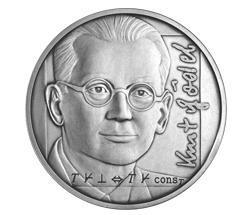
\includegraphics[width=3cm]{content/chapter_model_checking/cpachecker/images/goedel-medal}%
    \end{textblock*}%
    \bigskip
    \bigskip
    \bigskip
    \bigskip
  \item Used for Linux driver verification\\ with dozens of real bugs found and fixed in Linux
\end{itemize}
\end{frame}

% ---------------------------------------------------------------------

\begin{frame}{\cpacheckertitle: Concepts}
  \begin{itemize}
    \item Included Concepts:
    \begin{itemize}
      \item CEGAR
      \item Interpolation
      \item Adjustable-block encoding
      \item Conditional model checking
      \item Verification witnesses
    \end{itemize}
    \item Further available analyses:
    \begin{itemize}
      \item \impact algorithm
      \item Bounded model checking
      \item k-Induction
      \item Property-directed reachability
    \end{itemize}
  \end{itemize}
\end{frame}


% ---------------------------------------------------------------------

\begin{frame}{\cpacheckertitle: Concepts}
  \begin{itemize}
    \item Completely modular, and thus flexible and easily extensible
    \item Every abstract domain is implemented as a\\
    "Configurable Program Analysis" (CPA)
    \item E.g., predicate abstraction, explicit-value analysis, intervals, octagon, BDDs, memory graphs, and more
    \item Algorithms are central and implemented only once
    \item Separation of concerns
    \item Combined with Composite pattern
  \end{itemize}
\end{frame}

% ---------------------------------------------------------------------

\begin{frame}{\cpacheckertitle: Algorithms}
  \begin{itemize}
    \item CPAAlgorithm is the core algorithm\\ for reachability analysis / fixpoint iteration
    \item Other algorithms can be added if desired, e.g.,
    \begin{itemize}
      \item CEGAR
      \item Double-checking counterexamples
      \item Sequential combination of analyses
    \end{itemize}
  \end{itemize}
\end{frame}

% ---------------------------------------------------------------------

\begin{frame}[fragile]{\cpacheckertitle: Architecture}
  \resizebox{\textwidth}{!}{
    \documentclass[tikz]{standalone}
\usetikzlibrary{calc}
\usepackage{xspace}
\usepackage{xcolor}
\newcommand\definergbcolor[2]{\definecolor{#1}{rgb}{#2}}
\newcommand\definecmykcolor[2]{\definecolor{#1}{cmyk}{#2}}
\newcommand{\kinduction}{$k$-induction\xspace}
\newcommand{\kInduction}{$k$-Induction\xspace}
\begin{document}
\begin{tikzpicture}[line width=1pt]

\node[text width=1.5cm] (sourcecode) at ( 0cm,3.5cm) {\resizebox{1.5cm}{!}{\begin{tikzpicture}%
\draw[fill=black!10] (0,4) --(2.7,4) --(3.5,3.5) --(3.5,0) --(0,0) --cycle;%
\draw[fill=black!10] (2.7,4) --(2.7,3.5) --(3.5,3.5);%
\end{tikzpicture}%
}};
\node[text width=1.5cm,align=center] (sourcecode-label) at (sourcecode) {Source Code};

\node[text width=1.5cm] (spec) at ( 0cm,0cm) {\resizebox{1.5cm}{!}{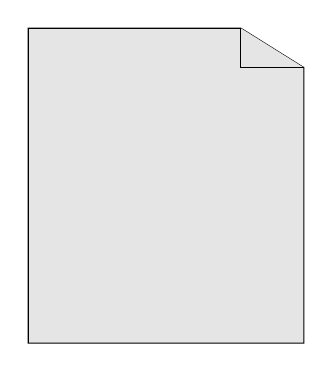
\begin{tikzpicture}%
\draw[fill=black!10] (0,4) --(2.7,4) --(3.5,3.5) --(3.5,0) --(0,0) --cycle;%
\draw[fill=black!10] (2.7,4) --(2.7,3.5) --(3.5,3.5);%
\end{tikzpicture}%
}};
\node[text width=1.5cm,align=center] (spec-label) at (spec) {Spec};

\node[text width=1.5cm] (results) at (10cm,3.5cm) {\resizebox{1.5cm}{!}{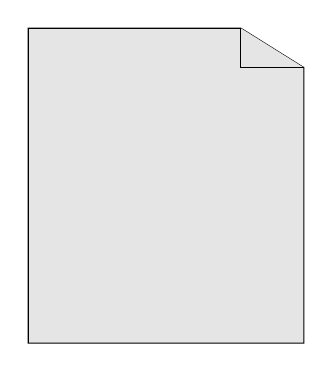
\begin{tikzpicture}%
\draw[fill=black!10] (0,4) --(2.7,4) --(3.5,3.5) --(3.5,0) --(0,0) --cycle;%
\draw[fill=black!10] (2.7,4) --(2.7,3.5) --(3.5,3.5);%
\end{tikzpicture}%
}};
\node[text width=1.5cm,align=center] (results-label) at (results) {Results};

\node[draw,text width=2cm,align=center,fill=sosyblue!20] (frontend)
 at (3cm, 3.5cm) {\mbox{Parser \&} \mbox{CFA Builder}};

\node[draw,text width=2cm,align=center,fill=green!60] (kindalgorithm)  at (6cm, 5.25cm) {\kinduction \mbox{Algorithm}};
\node[draw,text width=2cm,align=center,fill=green!60] (cegaralgorithm) at (6cm, 3.5cm) {CEGAR \mbox{Algorithm}};
\node[draw,text width=2cm,align=center,fill=green!60] (cpaalgorithm)   at (6cm, 1.75cm) {CPA \mbox{Algorithm}};

\node[draw,text width=1.5cm,align=center,fill=uniorange!60] (speccpa) at (3cm, 0cm) {Spec\\CPA};
\node[draw,text width=1.5cm,align=center,fill=uniorange!60] (loccpa) at (5cm, 0cm) {Location\\CPA};
\node[draw,text width=1.5cm,align=center,fill=uniorange!60] (callstackcpa) at (7cm, 0cm) {Callstack\\CPA};
\node[draw,text width=1.5cm, align=center,fill=uniorange!60] (predicatecpa) at (9cm, 0cm) {Predicate CPA};

\draw[->,double] (sourcecode) --(frontend);
\draw[->,double] (spec) --(speccpa);
\draw[->,double] (kindalgorithm) -|(results);
\draw[->,double] (cpaalgorithm) -|(results);

\draw[->] (frontend) |-(kindalgorithm);
\draw[->] (frontend) |-(cegaralgorithm);
\draw[->] (frontend) |-(cpaalgorithm);

\draw[->] (cpaalgorithm) --($(cpaalgorithm) - (0,0.75cm)$) -|(speccpa);
\draw[->] (cpaalgorithm) --($(cpaalgorithm) - (0,0.75cm)$) -|(loccpa);
\draw[->] (cpaalgorithm) --($(cpaalgorithm) - (0,0.75cm)$) -|(callstackcpa);
\draw[->] (cpaalgorithm) --($(cpaalgorithm) - (0,0.75cm)$) -|(predicatecpa);

\draw (kindalgorithm.south east) edge[bend left,->] (cpaalgorithm.north east);
\draw[->] (cegaralgorithm) --(cpaalgorithm);

\end{tikzpicture}
\end{document}

  }
\end{frame}

% ---------------------------------------------------------------------

% \begin{frame}{\resizebox{!}{7mm}{% Created with inkscape
\documentclass{standalone}
\usepackage{../sosy-beamer}

\begin{document}
\begin{tikzpicture}[y=0.80pt, x=0.80pt, yscale=-1.000000, xscale=1.000000, inner sep=0pt, outer sep=0pt]
\begin{scope}[shift={(-221.97172,-411.62445)}]
  \begin{scope}[shift={(174.94262,35.80334)}]
    % Checkmark
    \path[fill=green] (343.2732,431.6103) .. controls (346.6213,431.6104) and
      (349.1539,434.3576) .. (350.8709,439.8519) .. controls (354.3049,450.1540) and
      (356.7516,455.3050) .. (358.2111,455.3049) .. controls (359.3271,455.3050) and
      (360.0397,454.0001) .. (361.2416,452.2830) .. controls (385.3654,413.6505) and
      (449.4021,378.7382) .. (451.7061,377.1931) .. controls (453.5563,375.7472) and
      (455.2449,375.7948) .. (457.7931,375.8348) .. controls (460.5402,375.8350) and
      (465.3567,378.5405) .. (466.3841,379.8938) .. controls (467.9207,382.1169) and
      (468.9861,381.3650) .. (470.1138,389.0872) .. controls (468.5352,393.5092) and
      (467.3858,393.7940) .. (466.3207,394.8515) .. controls (427.1214,422.0592) and
      (392.8516,441.3973) .. (364.5211,485.6959) .. controls (362.5465,488.7865) and
      (358.5115,490.3318) .. (352.4162,490.3318) .. controls (346.2350,490.3318) and
      (342.5863,490.0743) .. (341.4703,489.5591) .. controls (338.5514,488.2714) and
      (335.1174,481.7039) .. (331.1683,469.8565) .. controls (326.7041,456.7215) and
      (324.4719,448.4799) .. (324.4720,445.1317) .. controls (324.4719,441.5261) and
      (327.4767,438.0491) .. (333.4863,434.7009) .. controls (337.1778,432.6406) and
      (340.4401,431.6104) .. (343.2732,431.6103);
    % Letter 'C'
    \path[fill=sosyblue] (119.3807,446.3865) -- (147.2947,454.8240) .. controls
      (145.4196,462.6522) and (142.4665,469.1912) .. (138.4354,474.4412) .. controls
      (134.4040,479.6912) and (129.3884,483.6521) .. (123.3885,486.3240) .. controls
      (117.4353,488.9959) and (109.8415,490.3318) .. (100.6072,490.3318) .. controls
      (89.4041,490.3318) and (80.2400,488.7146) .. (73.1150,485.4803) .. controls
      (66.0369,482.1990) and (59.9197,476.4568) .. (54.7635,468.2537) .. controls
      (49.6072,460.0506) and (47.0291,449.5506) .. (47.0291,436.7537) .. controls
      (47.0291,419.6913) and (51.5525,406.5897) .. (60.5994,397.4490) .. controls
      (69.6931,388.2616) and (82.5369,383.6679) .. (99.1307,383.6678) .. controls
      (112.1150,383.6679) and (122.3103,386.2929) .. (129.7166,391.5428) .. controls
      (137.1696,396.7928) and (142.7009,404.8553) .. (146.3104,415.7303) --
      (118.1854,421.9881) .. controls (117.2009,418.8475) and (116.1697,416.5506) ..
      (115.0916,415.0974) .. controls (113.3103,412.6600) and (111.1306,410.7850) ..
      (108.5525,409.4724) .. controls (105.9744,408.1600) and (103.0915,407.5038) ..
      (99.9041,407.5037) .. controls (92.6853,407.5038) and (87.1541,410.4100) ..
      (83.3104,416.2224) .. controls (80.4041,420.5350) and (78.9509,427.3084) ..
      (78.9510,436.5428) .. controls (78.9509,447.9803) and (80.6853,455.8318) ..
      (84.1541,460.0974) .. controls (87.6228,464.3162) and (92.4978,466.4256) ..
      (98.7791,466.4256) .. controls (104.8728,466.4256) and (109.4665,464.7147) ..
      (112.5604,461.2928) .. controls (115.7009,457.8709) and (117.9743,452.9022) ..
      (119.3807,446.3865);
    % Letter 'P'
    \path[fill=uniorange] (152.5188,387.2537) -- (205.4641,387.2537) .. controls
      (216.9953,387.2538) and (225.6203,389.9960) .. (231.3391,395.4803) .. controls
      (237.1046,400.9647) and (239.9874,408.7694) .. (239.9875,418.8943) .. controls
      (239.9874,429.3006) and (236.8468,437.4334) .. (230.5657,443.2928) .. controls
      (224.3312,449.1522) and (214.7922,452.0819) .. (201.9485,452.0818) --
      (184.5110,452.0818) -- (184.5110,490.3318) -- (152.5188,490.3318) --
      (152.5188,387.2537)(184.5110,431.1990) -- (192.3157,431.1990) .. controls
      (198.4562,431.1991) and (202.7687,430.1444) .. (205.2532,428.0349) .. controls
      (207.7375,425.8788) and (208.9797,423.1366) .. (208.9797,419.8084) .. controls
      (208.9797,416.5741) and (207.9016,413.8319) .. (205.7454,411.5818) .. controls
      (203.5891,409.3319) and (199.5344,408.2069) .. (193.5813,408.2068) --
      (184.5110,408.2068) -- (184.5110,431.1990);
    % Letter 'A'
    \path[fill=unigrey] (294.4918,473.3162) -- (258.2105,473.3162) --
      (253.2183,490.3318) -- (220.6636,490.3318) -- (259.4058,387.2537) --
      (294.1402,387.2537) -- (332.8824,490.3318) -- (299.5543,490.3318) --
      (294.4918,473.3162)(287.8121,451.0271) -- (276.4214,413.9724) --
      (265.1011,451.0271) -- (287.8121,451.0271);
  \end{scope}
\end{scope}

\end{tikzpicture}
\end{document}

}\enspace Try \cpachecker}
\begin{frame}{\cpacheckertitle: Try \cpachecker}
  \begin{itemize}
    \item Online at Google AppEngine:\\
    \url{https://cpachecker.appspot.com/}
    \item Download for Linux/Windows:\\
    \url{\cpacheckerurl}
    \begin{itemize}
      \item Run \texttt{scripts/cpa.sh} | \texttt{scripts$\backslash$cpa.bat}
      \item \texttt{-predicateAnalysis <FILE>}
      \item Windows/Mac need to disable bitprecise analysis:\\
        \texttt{-predicateAnalysis-linear\\ -setprop solver.solver=smtinterpol\\ -setprop analysis.checkCounterexamples=false}
    \end{itemize}
    \item Look at \texttt{output/CPALog.txt} for problems
    \item Open \texttt{.dot} files with dotty / xdot (\url{www.graphviz.org/})
    \item Open graphical report in browser: \texttt{output/*.html}
  \end{itemize}
\end{frame}

% ---------------------------------------------------------------------

\begin{frame}{\cpacheckertitle: Specification}
  \begin{itemize}
    \item Model Checkers check only what you specified
    \item \cpachecker's default:
    \begin{itemize}
      \item Label \texttt{ERROR}
      \item Calling function \_\texttt{assert\_fail()}
      \item \texttt{assert(pred)} needs to be pre-processed
    \end{itemize}
    \item SV-COMP:
    \begin{itemize}
      \item Calling function \_\texttt{VERIFIER\_error()}
      \item \texttt{-spec sv-comp-reachability}
    \end{itemize}
  \end{itemize}
\end{frame}

% ---------------------------------------------------------------------

\begin{frame}{\cpacheckertitle for Developers}
  Want to implement your own analysis?
  \begin{itemize}
    \item Easy, just write a CPA in Java
    \item Implementations for 10 interfaces needed
    \item But for 8, we have default implementations\\
      \textbf{$\rightarrow$} Minimal configuration: \\
      \qquad abstract state and\\
      \qquad abstract post operator
  \end{itemize}
\end{frame}

% ---------------------------------------------------------------------

\begin{frame}{\cpacheckertitle for Developers}
  The CPA framework is flexible:
  \begin{itemize}
    \item Many components are provided as CPAs:
      \begin{itemize}
        \item Location / program counter tracking
        \item Callstack tracking
        \item Specification input (as automata)
        \item Pointer-aliasing information
      \end{itemize}
    \item CPAs can be combined,\\
      so your analysis doesn't need to care about these things
  \end{itemize}
\end{frame}